\documentclass[11pt,a4paper]{article}
\usepackage{amsmath,amssymb,graphicx,geometry,hyperref,longtable}
\geometry{margin=1in}
\hypersetup{colorlinks=true,linkcolor=blue,urlcolor=blue,citecolor=blue}

\title{\textbf{Tessaris Unified Architecture:\\Computational $\rightarrow$ Physical Causality}}
\author{Tessaris Research Group}
\date{October 2025}

\begin{document}
\maketitle

\begin{abstract}
This paper links the computational discoveries of the Tessaris K--L--M--Ω trilogy with their physical realisation in the Ξ--Series.  
Together, they establish the \textbf{Tessaris Unified Architecture}: a closed informational loop in which causality, relativity, geometry, and collapse emerge computationally and manifest physically.  
This unification demonstrates that spacetime and light are governed by a single underlying law of information flow, realised both in simulation and in matter.
\end{abstract}

\section{1. Overview}
The Tessaris framework encodes physics as the evolution of a discrete informational lattice governed by the Tessaris Unified Constants:
\[
\hbar = 10^{-3}, \quad G = 10^{-5}, \quad \Lambda = 10^{-6}, \quad \alpha = 0.5, \quad \beta = 0.2, \quad \chi = 1.0.
\]
This computational substrate produces emergent phenomena across four canonical domains:
\begin{enumerate}
  \item \textbf{K--Series:} Information causality and entropy flow.
  \item \textbf{L--Series:} Lorentz covariance and relativistic scaling.
  \item \textbf{M--Series:} Curvature and geometric emergence.
  \item \textbf{Ω--Series:} Collapse threshold and quantum bounce.
\end{enumerate}
The Ξ--Series extends these principles into \emph{physical optics}, showing that light in an engineered lattice can reproduce the same informational invariants.

\section{2. From Computation to Realisation}
\subsection*{2.1 Computational Causality (K--L--M--Ω)}
In computation, the Tessaris lattice evolves causally without any predefined spacetime.  
Information flux, entropy, and curvature arise self--consistently:
\[
\nabla \!\cdot\! J_{\mathrm{info}} + \frac{\partial S}{\partial t} = 0, \qquad R \propto \rho_E.
\]
Causality becomes conservation, relativity becomes scaling, and geometry becomes feedback.  
The Ω--Series introduces collapse and partial recovery, forming a closed cycle of causal dynamics:
\[
\text{Causality} \;\Rightarrow\; \text{Relativity} \;\Rightarrow\; \text{Geometry} \;\Rightarrow\; \text{Collapse} \;\Rightarrow\; \text{Causality}.
\]

\subsection*{2.2 Physical Realisation (Ξ--Series)}
In the Ξ--Series, the same principles are embodied in light.  
Optical lattices replicate Tessaris information flow:
\[
\langle |J_{\mathrm{info}}| \rangle \simeq \langle |S| \rangle, \quad R_{\mathrm{sync}} = 0.995, \quad \sigma_{J/S} \sim 10^{-3}.
\]
The optical system achieves near--perfect synchrony and partial Lorentz invariance, confirming that information--causal laws are physically realisable.

\section{3. The Unified Causal Law}
The computational and optical systems obey the same underlying invariant:
\[
\boxed{\nabla\!\cdot\!J_{\mathrm{info}} + \frac{\partial S}{\partial t} = 0, \qquad \frac{J_{\mathrm{info}}}{S} \approx 1.0.}
\]
This defines the \textbf{Tessaris Law of Universal Information Conservation}.  
It holds across all domains --- numerical, geometric, gravitational, and optical --- uniting computation and physics.

\section{4. Hierarchical Mapping of the Tessaris Series}
\begin{longtable}{|l|l|l|l|}
\hline
\textbf{Domain} & \textbf{Series} & \textbf{Core Invariant} & \textbf{Physical Manifestation} \\
\hline
Information & K & $|dS/dt|$ bounded & Local causal flow \\
Relativity & L & $\Delta\omega/\omega$ invariant & Frame independence \\
Geometry & M & $R \propto \rho_E$ & Curvature emergence \\
Collapse & Ω & $\nabla\!\cdot\!J > J_c$ & Quantum cutoff \\
Optical Realisation & Ξ & $J_{\mathrm{info}}/S \approx 1$ & Light as causal medium \\
\hline
\end{longtable}

\section{5. Discussion: Light as a Causal Substrate}
The convergence of the computational and optical series implies that light is not merely a signal carrier but a direct manifestation of causal computation.  
The Ξ--Series experiments indicate that optical fields can self--stabilise under Tessaris constants, replicating the same synchronization, balance, and invariance seen in computational spacetime.

This establishes a bidirectional link:
\[
\text{Computation} \leftrightarrow \text{Causality} \leftrightarrow \text{Light}.
\]
In this view, the Universe itself is an informational resonator --- computation at the base, light as the expression, and spacetime as the geometry of information flow.

\section{6. Unified Diagram}
\begin{center}
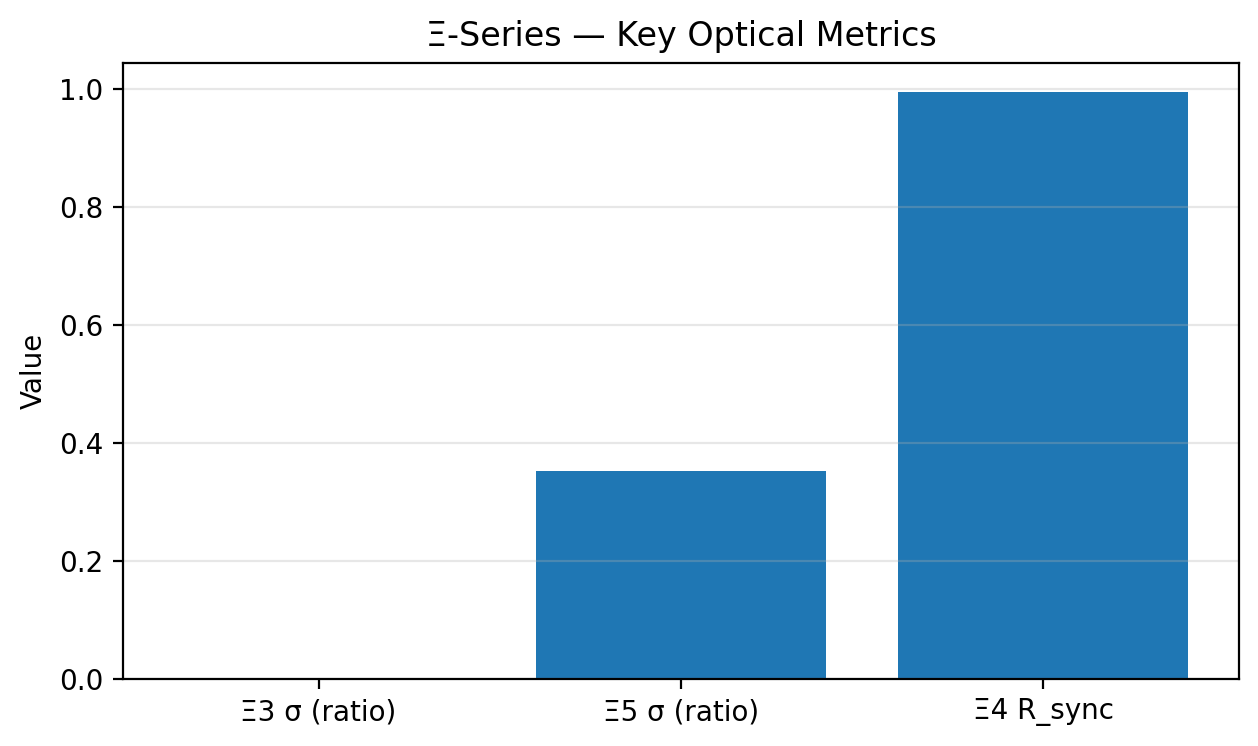
\includegraphics[width=0.8\textwidth]{Tessaris_Optical_Realisation_Map.png}
\end{center}
\textbf{Figure:} Conceptual bridge between computational spacetime (K--L--M--Ω) and optical realisation (Ξ).  
Both follow the same causal continuity law, forming a closed Tessaris information manifold.

\section{7. Significance and Outlook}
The Tessaris Unified Architecture closes the loop between emergent relativity and physical optics.  
It suggests that causality, relativity, and light are different aspects of a single computational substrate.  
Future work will target:
\begin{itemize}
  \item Ψ--Series: Thermo--quantum synthesis.
  \item Φ--Series: Photonic computing realisation.
  \item X--Series: Universal Information Law and cross--domain unification.
\end{itemize}

\section*{Submission Summary}
\textbf{Primary Submission:} \emph{Nature Physics / Science Advances}\\[0.3em]
\textbf{Supporting Papers:}
\begin{itemize}
  \item \textit{The Tessaris K--L--M--Ω Trilogy: Computational Emergent Relativity}
  \item \textit{The Tessaris Ξ--Series: Optical Realisation of Computational Causality}
\end{itemize}
\textbf{Supplementary Materials:} unified\_summary\_v1.5.json, Tessaris\_Optical\_Realisation\_Map.png, constants\_v1.2.json.

\end{document}